\section{Introduction}

BGP is the critical infrastructure for the Internet and interdomain routing.  The routing protocol operates in the junction point where independent networks (an AS, or autonomous system) exchange network traffic through proscribed and announced routes of connectivity.  Because ASes are separate networking and economic entities, BGP must operate balancing essentially two purposes, which are not entirely orthogonal to each other: the limits of efficient networked traffic and the realities of routing policies, which are governed by cost expenses, some issues of politics, network locality, and multihoming preferences.  These have served together, and at times as trade-offs, to add to complexity within BGP and to bring the level of routed Internet traffic -- with its number of policy-constrained routing inefficiencies -- such as is seen at this time.

As originally envisioned, a hierarchical and scalable routing table was to serve as an efficient and streamlined mechanism.  However, not foreseen was how the limited number of IPv4 addresses ($2^{32}$) and the increasing number of allocations to users would lead to fractionalization and finer segmentation of the IP address space.  Fragmentation has effectively flattened portions of the IP address table, rather than preserved the hierarchical IP address-based routing.  Reasons for numerous "special-case" announcements include multihoming demands and Internet customers' implementation of particular traffic engineering to suit any special purposes.  Likewise, single institutions have grown to need more IP addresses than originally allocated and have received additional address blocks that are non-adjacent.  In either case, it has generated a routing table with more entries than a hierarchical structure would have yielded that strictly worked with consolidated blocks.  Correspondingly, the Internet experiences a higher number of transmitted BGP updates to propagate these steadily ongoing changes.  

Several issues impact the growth of the BGP routing table.  First is the challenge of best guessing

\begin{figure}[htbp]
	\centering
		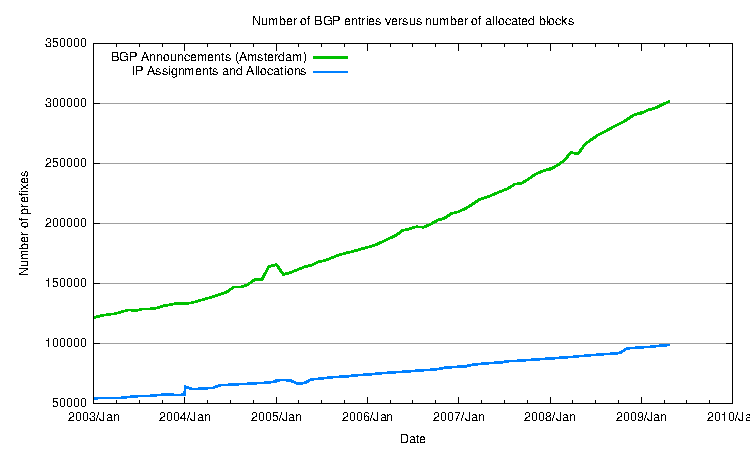
\includegraphics[width=\columnwidth]{01_bgp_ip_size/02_bgp_max_vs_ip}
	\caption{Average number of BGP entries versus number of allocated IP blocks}
	\label{fig:BGP vs RIR}
\end{figure}

\begin{figure}[htbp]
	\centering
		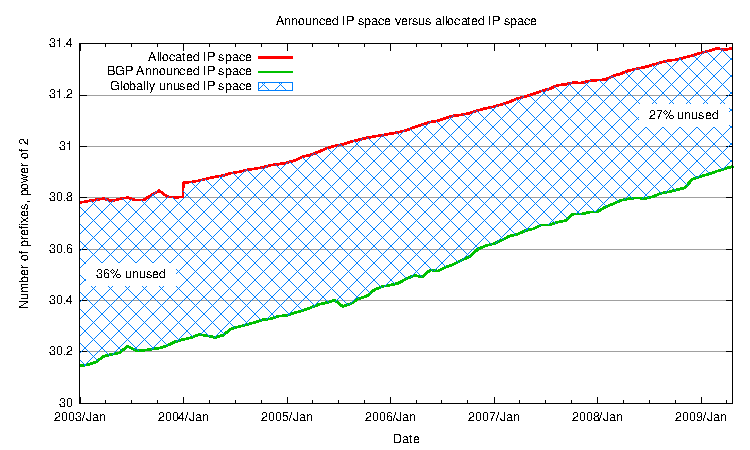
\includegraphics[width=\columnwidth]{01_bgp_ip_size/02_bgp_max_vs_ip_space}
	\caption{Average number of BGP announced IP space versus allocated IP space}
	\label{fig:BGP vs RIR space}
\end{figure}
% The existing Internet fully relies on the BGP protocol~\cite{Rekhter:1995:RFC1771-BGP} to maintain global connectivity. The key element of the BGP is that each participant (autonomous system, AS) announces its IP prefixes which are propagated to the rest of the ASes by means of the protocol. Although the announced set is generally limited by the address blocks allocated to a particular AS by a Regional Internet Registry (RIR), the AS itself decides the granularity of the announcements. In other words, ASes having only one allocated address block can announce multiple prefixes. The two major reasons for this are traffic engineering and multihoming. The popularity of this prefix splitting can be demonstrated by allocation vs announcement statistics. The number of announced prefixes (160K in 2004~\cite{Meng:2005:IPv4-address} growing 300K in 2009~\cite{::BGP-Reports}) is more than two times the number of allocated IPv4 blocks (65K in 2004, 140K in 2009 respectively). These dynamics cast doubt on global routing scalability.
% 
% As originally envisioned, a hierarchical and scalable routing table was to serve as an efficient and streamlined mechanism. However, not foreseen was how the limited number ($2^{32}$) of IPv4 addresses and alongside the increasing number of allocations to users would lead to fractionalization and finer segmentation of the IP address table. There exist several solutions which attempt to contain the size of the global routing table.  Accompanying the growth of the IP assignments have been aggregation techniques with the intent to gather a group of prefixes under a more general IP prefix. However, Internet customers with particular traffic engineering and multihoming demands have preferred that these guidelines not be implemented. On the other hand, some customers willing to aggregate are not in a position to do so, due to the inability of RIRs to assign a specific requester a contiguous range of IP addresses. Such is the case, for example, with UCLA which has accumulated eight IPv4 address blocks and is forced to announce eight different prefixes (128.97.0.0/16, 131.179.0.0/16, 149.142.0.0/16, 164.67.0.0/16, 169.232.0.0/16, 192.35.210.0/24, 192.35.225.0/24, 192.154.2.0/24). This granular allocation has been one of the major contributors to the growth of the global routing table. An interesting topic to pursue would be to find the average number of allocated blocks assigned to various ASes.
% 
% Meng et al.~\cite{Meng:2005:IPv4-address} reported a number of statistics that will serve as a baseline for our project.  These include 1) the number of allocated blocks and 2) the number of announced prefixes. We propose to conduct more detailed research by country and AS granularity on the ratio and correlation between the number of allocated blocks and the announced prefixes within the BGP routing table. Arguably, any attempt to renumber allocations such that they are less fragmented would reduce both the number of allocations and correspondingly the number of prefixes and size of the BGP table. Our analysis will help to establish an upper bound of the potential BGP routing table reduction if an IPv4 renumbering technique were to be implemented. Additionally, this will justify the necessity of effective IPv6 address assignment and reassignment techniques.

% picture of total # of prefixes
% picture of total # of IP space



The paper is organized as follows.  Section~\ref{sec:data sets} describes the data sets and methodology used in our study.

% Section~\ref{sec:} provides an introduction to the Border Gateway Protocol.    Section 4 presents statistics for IP address allocation and announcement and the BGP table growth.  Section 5 concerns the trends of fragmentation in the BGP routing table.  Section 6 draws a connection between locality and routing table growth, and it shows in which parts of the globe Internet connectivity has been expanding over the last several years.  Section 7 presents data on the longevity and stability of routing table entries.  Related work is discussed in Section 8, followed by the conclusion in Section 9.